\documentclass[]{scrreprt}   % list options between brackets        
\usepackage{graphicx, listings, color}      % list packages between braces
\graphicspath{ {images/} }

% type user-defined commands here

\definecolor{codegreen}{rgb}{0,0.6,0}
\definecolor{codegray}{rgb}{0.5,0.5,0.5}
\definecolor{codepurple}{rgb}{0.58,0,0.82}
\definecolor{backcolour}{rgb}{0.95,0.95,0.92}

\lstdefinestyle{mystyle}{
	backgroundcolor=\color{backcolour},   
	commentstyle=\color{codegreen},
	keywordstyle=\color{magenta},
	numberstyle=\tiny\color{codegray},
	stringstyle=\color{codepurple},
	basicstyle=\footnotesize,
	breakatwhitespace=false,         
	breaklines=true,                 
	captionpos=b,                    
	keepspaces=true,                 
	numbers=left,                    
	numbersep=5pt,                  
	showspaces=false,                
	showstringspaces=false,
	showtabs=false,                  
	tabsize=2
}

\lstset{style=mystyle}

\begin{document}
	
\title{CAB420 Assignment 1}   % type title between braces
\author{Aidan Kinzett (n9699210)}         % type author(s) between braces
\maketitle
\chapter{Theory}

Given the following equation,

$$L(w)=-\sum_{i=1}^{N}log(\frac{1}{1+e^{y_i(w^Tx_i+b)}})+\lambda||w||_2^2$$

\section{Finding the Partial Derivative}
Finding the partial derivative $$\frac{\partial L}{\partial w_j}$$

$$\frac{\partial L}{\partial w_j}(-\sum_{i=1}^{N}log(\frac{1}{1+e^{y_i(w^Tx_i+b)}})+\lambda||w||_2^2)$$

As the part at the end of the function is a squared L2 norm, it can be derived as below.

$$\frac{\partial L}{\partial w_j}(-\sum_{i=1}^{N}log(\frac{1}{1+e^{y_i(w^Tx_i+b)}}))+2\lambda w_j$$

Simplify,

$$\frac{\partial L}{\partial w_j}(\sum_{i=1}^{N}log(1+e^{y_i(w^Tx_i+b)}))+2\lambda w_j$$

Chain rule,

$$\sum_{i=1}^{N}\frac{\frac{\partial L}{\partial w_j}(1+e^{y_i(w^Tx_i+b)})}{1+e^{y_i(w^Tx_{i,j}+b)}}+2\lambda w_j$$

$$\sum_{i=1}^{N}\frac{\frac{\partial L}{\partial w_j}(1)+\frac{\partial L}{\partial w_j}(e^{y_i(w^Tx_i+b)})}{1+e^{y_i(w^Tx_{i,j}+b)}}+2\lambda w_j$$

$$\sum_{i=1}^{N}\frac{\frac{\partial L}{\partial w_j}(e^{y_i(w^Tx_i+b)})}{1+e^{y_i(w^Tx_{i,j}+b)}}+2\lambda w_j$$

Chain rule,

$$\sum_{i=1}^{N}\frac{y_ix_ie^{y_i(w^Tx_i+b)}}{1+e^{y_i(w^Tx_{i,j}+b)}}+2\lambda w_j$$

\section{Finding the Second Partial Derivative}
Finding the second partial derivative $$\frac{\partial^2 L}{\partial w_j\partial w_k}$$

$$\frac{\partial^2 L}{\partial w_j\partial w_k}=\frac{\partial}{\partial w_k}(\sum_{i=1}^{N}\frac{y_ix_ie^{y_i(w^Tx_i+b)}}{1+e^{y_i(w^Tx_{i,j}+b)}}+2\lambda w_j)$$


$$\sum_{i=1}^{N}\frac{y_ix_i(\frac{\partial}{\partial w_k}e^{y_i(w^Tx_i+b)})}{1+e^{y_i(w^Tx_{i,j}+b)}}$$

Using the chain rule,

$$\sum_{i=1}^{N}\frac{e^{y_i(w_kx_i+b)}y_i^2x_i(\frac{\partial}{\partial w_k}(w^Tx_i+b))}{1+e^{y_i(w^Tx_{i,j}+b)}}$$

$$\sum_{i=1}^{N}\frac{e^{y_i(w^Tx_i+b)}y_i^2x_iw_kx_i+b}{1+e^{y_i(w^Tx_{i,j}+b)}}$$

$$\sum_{i=1}^{N}\frac{e^{y_i(w^Tx_i+b)}y_i^2x_i^2w_k+b}{1+e^{y_i(w^Tx_{i,j}+b)}}$$


\section{Proving it's a convex function}

A function can be defined as convex if the Hessian matrix is positive semi-definite. This is defined as,

$$a^THa\equiv\sum_{j,k}a_ja_kH_{j,k}\geq0$$

Where,

$$H_{j,k}=\frac{\partial^2L}{\partial w_j\partial w_k}$$

This could be shown by contradiction.
\chapter{Practice}

\section{Features, Classes, and Linear Regression (10 Marks)}
\textbf{a) Plot the training data in a scatter plot.}
\begin{center}
	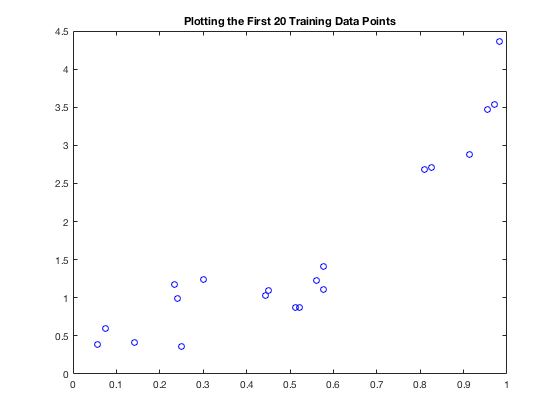
\includegraphics[width=30em,keepaspectratio]{p1figure1.png}\\
	{Figure 2.1.1: Training data in a scatter plot.}
\end{center} 

\textbf{b) Create a linear regression learner using the above functions. Plot it on the same plot as the training data.}
\begin{center}
	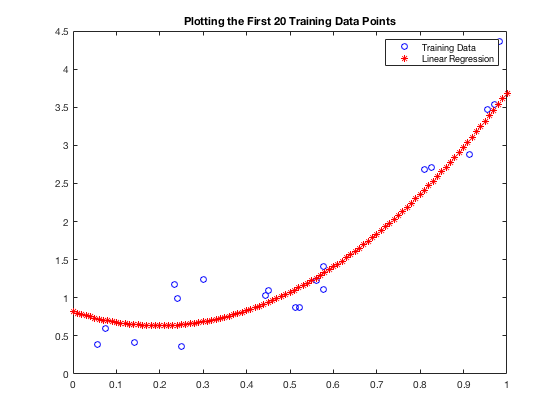
\includegraphics[width=30em,keepaspectratio]{p1figure2.png}\\
	{Figure 2.1.2: Training data in a scatter plot with linear regression learner}
\end{center} 

\textbf{(c) Create plots with the data and a higher-order polynomial (3, 5, 7, 9, 11, 13).}
\begin{center}
	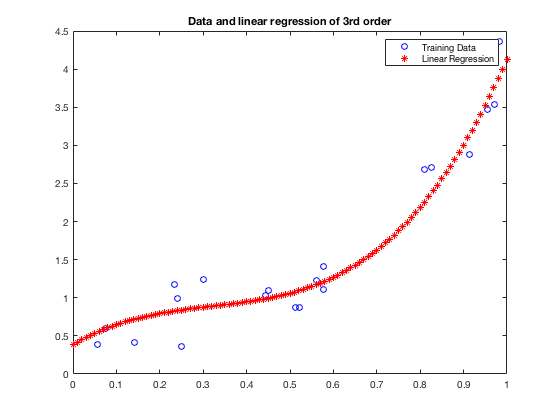
\includegraphics[width=30em,keepaspectratio]{p1figure3.png}\\
	{Figure 2.1.3: Training data in a scatter plot with 3rd order linear regression learner}
	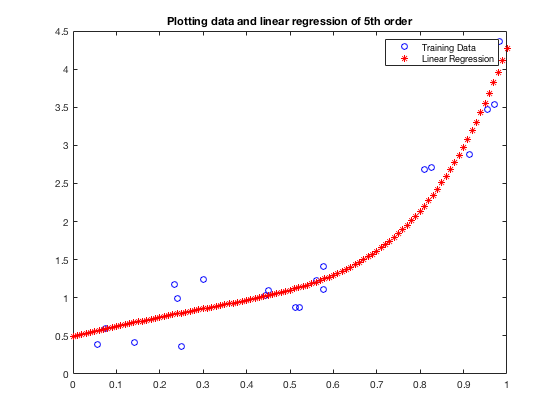
\includegraphics[width=30em,keepaspectratio]{p1figure4.png}\\
	{Figure 2.1.4: Training data in a scatter plot with 5th order linear regression learner}
	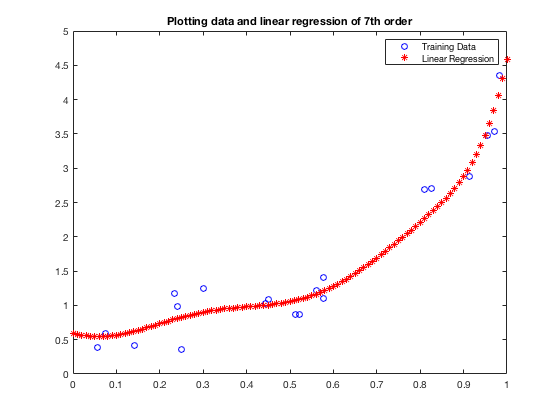
\includegraphics[width=30em,keepaspectratio]{p1figure5.png}\\
	{Figure 2.1.5: Training data in a scatter plot with 7th order linear regression learner}
	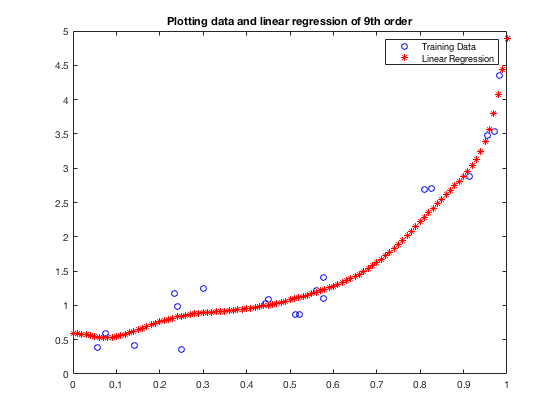
\includegraphics[width=30em,keepaspectratio]{p1figure6.png}\\
	{Figure 2.1.6: Training data in a scatter plot with 9th order linear regression learner}
	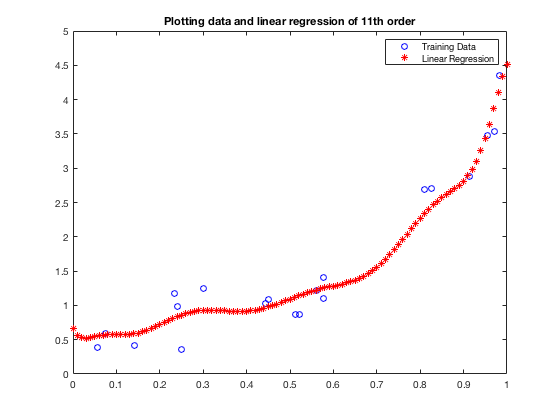
\includegraphics[width=30em,keepaspectratio]{p1figure7.png}\\
	{Figure 2.1.7: Training data in a scatter plot with 11th order linear regression learner}
	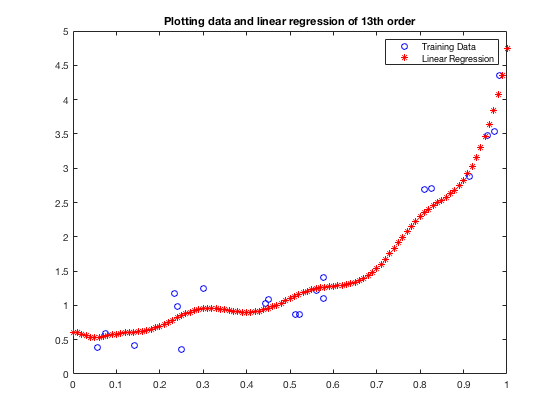
\includegraphics[width=30em,keepaspectratio]{p1figure8.png}\\
	{Figure 2.1.8: Training data in a scatter plot with 13th order linear regression learner}
\end{center} 

\textbf{(d) Calculate the mean squared error (MSE) associated with each of your learned models on the training data.}

\begin{verbatim}
Training MSE of order 2 regression
tr_err =
0.1092

Training MSE of order 3 regression
tr_err =
0.0828

Training MSE of order 5 regression
tr_err =
0.0813

Training MSE of order 7 regression
tr_err =
0.0783

Training MSE of order 9 regression
tr_err =
0.0771

Training MSE of order 11 regression
tr_err =
0.0756

Training MSE of order 13 regression
tr_err =
0.0750
\end{verbatim}

\textbf{(e) Calculate the MSE for each model on the test data (in mTestData.txt).}

\begin{verbatim}
Testing MSE of order 2 regression
te_err =
0.0972

Testing MSE of order 3 regression
te_err =
0.0983

Testing MSE of order 5 regression
te_err =
0.0959

Testing MSE of order 7 regression
te_err =
0.1094

Testing MSE of order 9 regression
te_err =
0.1135

Testing MSE of order 11 regression
te_err =
0.1132

Testing MSE of order 13 regression
te_err =
0.1128
\end{verbatim}

\textbf{(f) Calculate the MAE for each model on the test data. Compare the obtained MAE values with the MSE values obtained in above (e).}

\begin{verbatim}
MAE for order 2 regression
te_mae =
0.2599

MAE for order 3 regression
te_mae =
0.2777

MAE for order 5 regression
te_mae =
0.2745

MAE for order 7 regression
te_mae =
0.2889

MAE for order 9 regression
te_mae =
0.2919

MAE for order 11 regression
te_mae =
0.2940

MAE for order 13 regression
te_mae =
0.2925
\end{verbatim}

{The MSE on test data and the MAE both increase in the same manner with the increase in order. The MAE values are larger, which is to be expected. Visually, they both seem to be accurate representations of the amount of error, and the differences in values match the differences in the  graphs.}
\bigbreak
\textbf{(g) Don’t forget to label your plots; see help legend.}
{The graphs have appropriate labelling.}

\section{kNN Regression (15 Marks)}
\textbf{(a) Using the knnRegress class, implement (add code to) the predict function to make it functional.}

\lstinputlisting[language=Matlab]{MATLABfiles/@knnRegress/predict.m}
\bigbreak
\textbf{(b) Using the same technique as in Problem 1a, plot the predicted function for several values of k : 1, 2, 3, 5, 10, 50. How does the choice of k relate to the “complexity” of the regression function?}

\begin{center}
	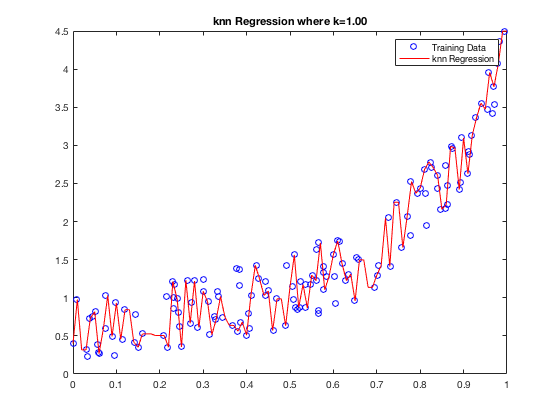
\includegraphics[width=30em,keepaspectratio]{p2figure1.png}\\
	{Figure 2.2.1: Predicted function for k=1.}
	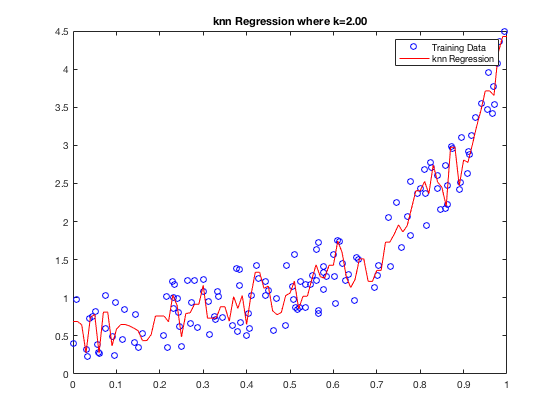
\includegraphics[width=30em,keepaspectratio]{p2figure2.png}\\
	{Figure 2.2.2: Predicted function for k=2.}
	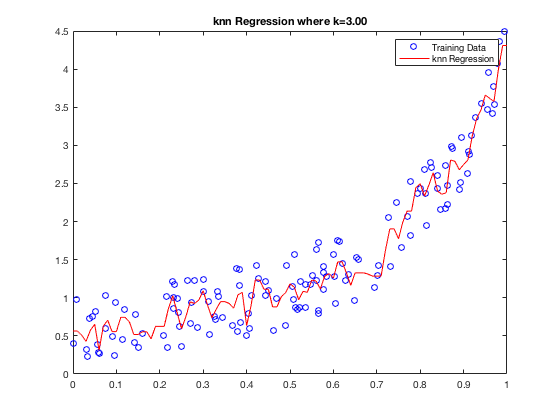
\includegraphics[width=30em,keepaspectratio]{p2figure3.png}\\
	{Figure 2.2.3: Predicted function for k=3.}
	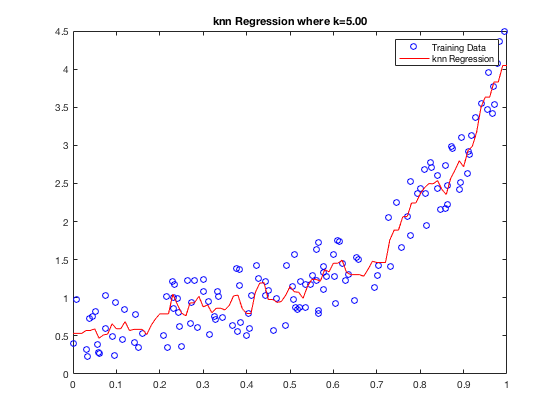
\includegraphics[width=30em,keepaspectratio]{p2figure4.png}\\
	{Figure 2.2.4: Predicted function for k=5.}
	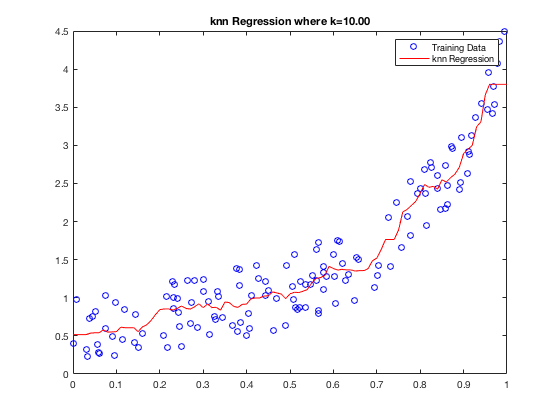
\includegraphics[width=30em,keepaspectratio]{p2figure5.png}\\
	{Figure 2.2.5: Predicted function for k=10.}
	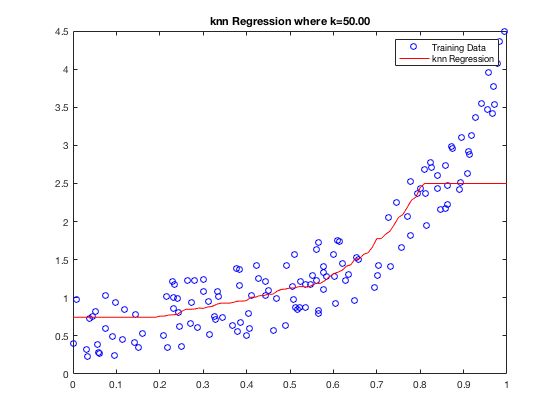
\includegraphics[width=30em,keepaspectratio]{p2figure6.png}\\
	{Figure 2.2.6: Predicted function for k=50.}
\end{center} 
\bigbreak
{The regression is more complex with lower k values, and less complex with higher k values. When k is low the regression is only looking at one piece of data, so jumps around with the data. When k is high it is looking at a lot of the data, and as a result doesn't follow the data very well. }
\bigbreak
\textbf{(c) We discussed in class that the k-nearest-neighbor classifier’s decision boundary can be shown to be piecewise linear. What kind of functions can be output by a nearest neighbor regression function? Briefly justify your conclusion. (You do not need to discuss the general case – just the 1-dimensional regression picture such as your plots.)}
\bigbreak
{For most cases, including this one, the output function will be piecewise linear. It is linear as there is only one y value for each x value. Its piecewise because its not able to be plotted as a single function due to how complex it is.}

\section{Hold-out and Cross-validation (15 Marks)}
\textbf{(a) Similarly to Problem 1 and 2, compute the MSE of the test data on a model trained on only the first 20 training data examples for k = 1, 2, 3, . . . , 140. Plot both train and test MSE versus k on a log-log scale (see help loglog). Assign title to your figure (ie. 20 data) and legends to your curves (ie. test, train). Discuss what you observed from the figure.}

\begin{center}
	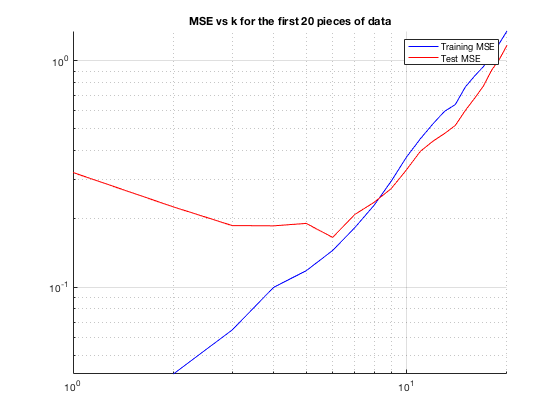
\includegraphics[width=30em,keepaspectratio]{p3figure1.png}\\
	{Figure 2.3.1: Train and test MSE versus k on a log-log scale.}
\end{center} 

{The regression is overfitted to the training data with low k values, then as the k value goes up both sets of data because similarly well fitted, then start increasing in error.}

\textbf{(b) Repeat, but use all the training data. What happened? Contrast with your results from Problem 1 (hint: which direction is “complexity” in this picture?).}

\begin{center}
	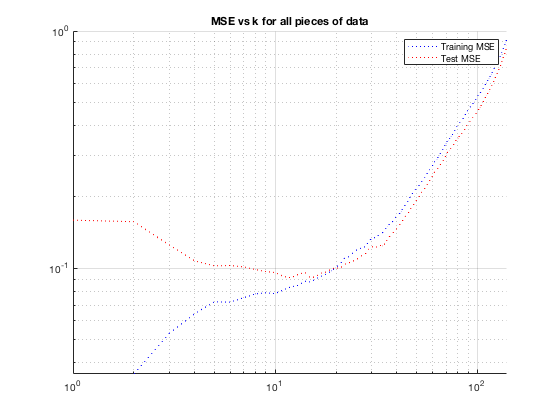
\includegraphics[width=30em,keepaspectratio]{p3figure2.png}\\
	{Figure 2.3.2: Train and test MSE versus k on a log-log scale.}
\end{center} 

{The two sets of data start to have a steeper increase in MSE as k increases. The functions keep getting less and less complex, and increase in error.}

\textbf{(c) Using only the training data, estimate the curve using 4-fold cross-validation. Split the training data into two parts, indices 1:20 and 21:140; use the larger of the two as training data and the smaller as testing data, then repeat three more times with different sets of 20 and average the MSE. Plot this together with (a) and (b). Use different colors or marks to differentiate three scenarios. Discus why might we need to use this technique via comparing curves of three scenario?}

\begin{center}
	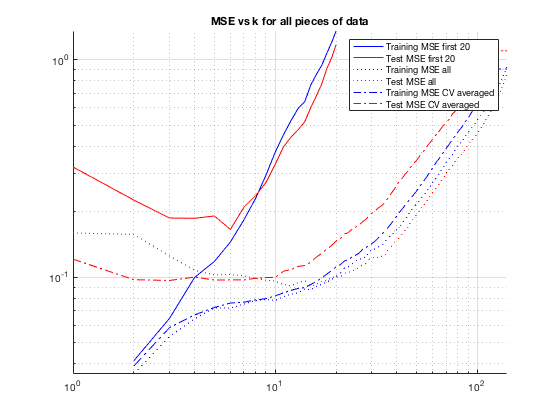
\includegraphics[width=30em,keepaspectratio]{p3figure3.png}\\
	{Figure 2.3.3: MSE of different techniques versus k on a log-log scale.}
\end{center} 

{The cross validation allows us to get an estimated accuracy by averaging out the accuracy from multiple models.}

\section{Nearest Neighbor Classifiers (15 Marks)}
\textbf{(a) Plot the data by their feature values, using the class value to select the color.}
\begin{center}
	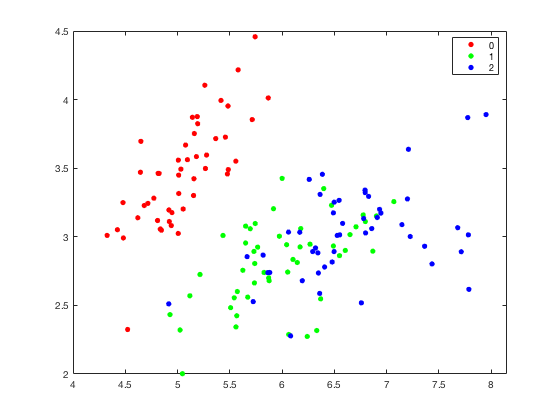
\includegraphics[width=30em,keepaspectratio]{p4figure1.png}\\
	{Figure 2.4.1:Plotted data by feature value with coloured classes}
\end{center} 
\textbf{(b) Use the provided knnClassify class to learn a 1-nearest-neighbor predictor. Use the function class2DPlot(learner,X,Y) to plot the decision regions and training data together.}
\begin{center}
	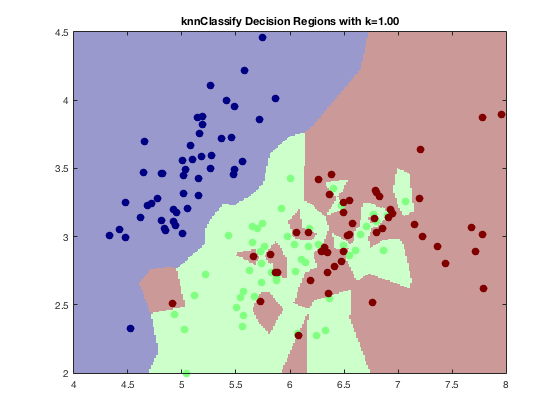
\includegraphics[width=30em,keepaspectratio]{p4figure2.png}\\
	{Figure 2.4.2:Plotted data with decision region for k=1}
\end{center} 

\textbf{(c) Do the same thing for several values of k (say, [1, 3, 10, 30]) and comment on their appearance.}
\begin{lstlisting}[language=Matlab]
	for k=[1, 3, 10, 30]
	learner = knnClassify(k, X, Y);
	class2DPlot(learner, X, Y);
	title(sprintf('knnClassify Decision Regions with k=%.2f',k));
	end
\end{lstlisting}
\begin{center}
	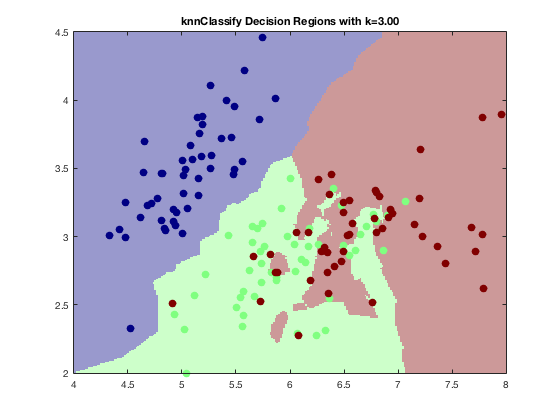
\includegraphics[width=30em,keepaspectratio]{p4figure3.png}\\
	{Figure 2.4.3:Plotted data with decision region for k=3}
\end{center} 
\begin{center}
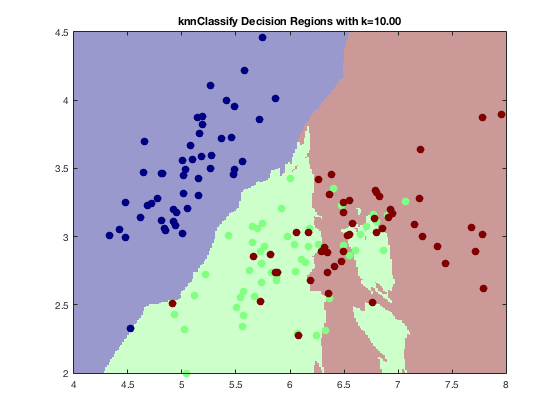
\includegraphics[width=30em,keepaspectratio]{p4figure4.png}\\
{Figure 2.4.4:Plotted data with decision region for k=10}
\end{center} 
\begin{center}
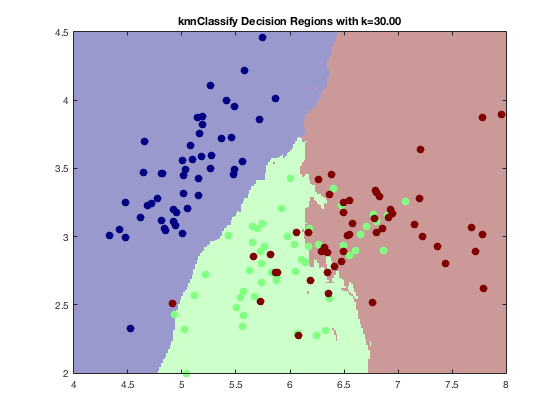
\includegraphics[width=30em,keepaspectratio]{p4figure5.png}\\
{Figure 2.4.5:Plotted data with decision region for k=30}
\end{center} 
\bigbreak
{In these graphs small values of k (such as 1) look to be over fitted, with many regions, while larger values (such as 30) are underfitting with a single region. This is for similar reasons as the regression in Section 2. The most appropriate fit appears to be when k=3. }

\bigbreak

\textbf{(d) Now split the data into an 80/20 training/validation split. For k = [1, 2, 5, 10, 50, 100, 200], learn a model on the 80$\%$ and calculate its performance ($\#$ of data classified incorrectly) on the validation data. What value of k appears to generalize best given your training data? Comment on the performance at the two endpoints, in terms of over- or under-fitting.}

\begin{lstlisting}[language=Matlab]
testp = randperm(size(iris,1), ceil(size(iris,1)/5));
trainp = setdiff(1:size(iris,1), testp);

training = iris(testp, :);
testing = iris(trainp, :);

kvalues = [1, 2, 5, 10, 50, 100, 200];
err = zeros(length(kvalues), 1);

for i = 1:length(kvalues)
learner = knnClassify(kvalues(i), training(:, 1:4), training(:, 5));
Yhat = predict(learner, testing(:, 1:4));

err(i) = sum(Yhat(:) ~= testing(:,5));
end

plot(kvalues, err, 'b*-')
title('Perfomance of different k values');
\end{lstlisting}
\begin{center}
	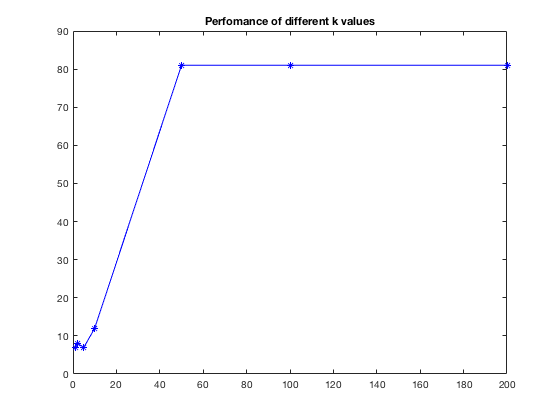
\includegraphics[width=30em,keepaspectratio]{p4figure6.png}\\
	{Figure 2.4.6:Performance for different k values}
\end{center} 
\bigbreak
{The k value with the least error in this case is k=6. k=1 is slightly overfitting the training data, and causing error when tested against the test data. k=50 up to k=200 are massively underfitting the data, and causing a lot of errors. }

\section{Perceptrons and Logistic Regression (25 Marks)}

\textbf{(a) Show the two classes in a scatter plot and verify that one is linearly separable while the other is not.}
\begin{center}
	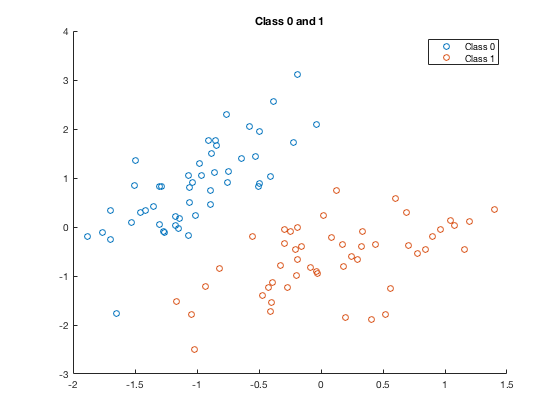
\includegraphics[width=30em,keepaspectratio]{p5figure1.png}\\
	{Figure 2.5.1: The data is separable as it is in two distinct groups}
		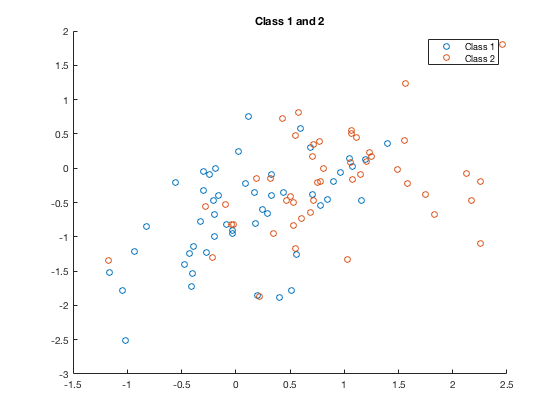
\includegraphics[width=30em,keepaspectratio]{p5figure2.png}\\
	{Figure 2.5.2: This data is not separable as it is mixed in with each other, not in well defined groups}
\end{center} 

\textbf{(b) Write ( fill in) the function @logisticClassify2/plot2DLinear.m so that it plots the two classes of data in different colors, along with the decision boundary (a line). Include the listing of your code in your report.}

\lstinputlisting[language=Matlab]{MATLABfiles/@logisticClassify2/plot2DLinear.m}
\bigbreak

\textbf{To demo your function plot the decision boundary corresponding to the classifier $sign(.5 + 1x 1 - .25x 2 )$ along with the A data, and again with the B data.}

\begin{lstlisting}[language=Matlab]
learner = logisticClassify2(); % create "blank" learner 
learner = setClasses(learner, unique(YA)); % define class labels using YA or YB 
wts = [0.5 1 -0.25]; 
learner = setWeights(learner, wts); % set the learner's parameters
plot2DLinear(learner, XA, YA);

figure;
learner2 = logisticClassify2(); % create "blank" learner 
learner2 = setClasses(learner2, unique(YB)); % define class labels using YA or YB 
wts = [0.5 1 -0.25]; 
learner2 = setWeights(learner2, wts); % set the learner's parameters
plot2DLinear(learner2, XB, YB);
\end{lstlisting}
\bigbreak
\begin{center}
	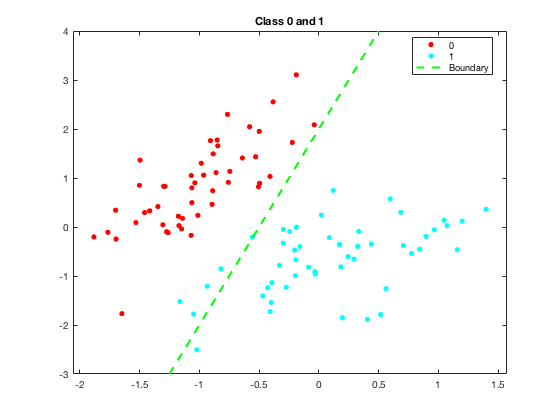
\includegraphics[width=30em,keepaspectratio]{p5figure3.png}\\
	{Figure 2.5.3: Classes and decision boundary}
	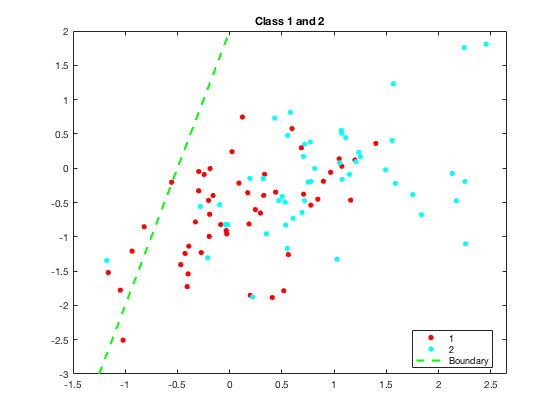
\includegraphics[width=30em,keepaspectratio]{p5figure4.png}\\
	{Figure 2.5.4: Classes and decision boundary}
\end{center} 

\textbf{(c) Complete the predict.m function to make predictions for your linear classifier.}

\lstinputlisting[language=Matlab]{MATLABfiles/@knnClassify/predict.m}

\bigbreak

\textbf{Again, verify that your function works by computing \& reporting the error rate of the classifier in the previous part on both data sets A and B. (The error rate on data set A should be ~ 0.0505.)}

\begin{verbatim}
errA =
0.0505

errB =
0.4646
\end{verbatim}

\textbf{You can also test this and your previous function by comparing your plot2DLinear output with the generic plotClassify2D function, which shows the decision boundary “manually” by calling predict on a dense grid of locations, rather than analytically as your plot2DLinear function should do.}

\begin{center}
	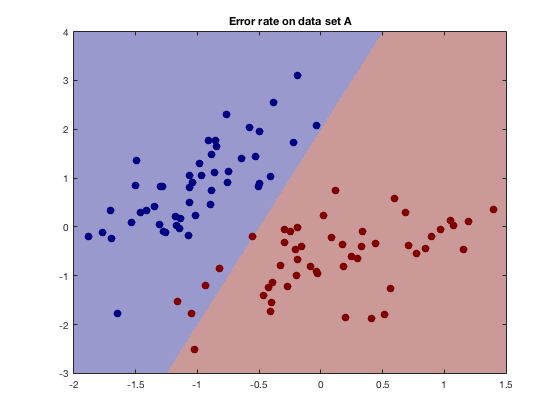
\includegraphics[width=30em,keepaspectratio]{p5figure5.png}\\
	{Figure 2.5.5: Classes and decision boundary plotted using plotClassify2D}
	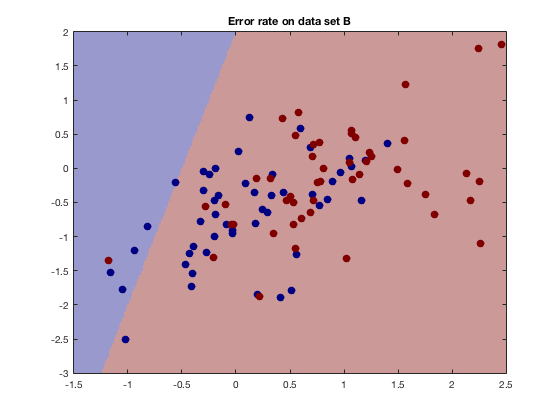
\includegraphics[width=30em,keepaspectratio]{p5figure6.png}\\
	{Figure 2.5.6: Classes and decision boundary plotted using plotClassify2D}
\end{center} 

\textbf{(d) In my provided code, I first transform the classes in the data Y into "class 0" (negative) and "class 1" (positive). In our notation, let $z = \theta x^{(i)}$ is the linear response of the perceptron, and $\sigma$ is the standard logistic function.
	$$\sigma (z) = (1 + exp(-z))^{-1}$$
	The (regularized) logistic negative log likelihood loss for a single data point j is then
	$$ J_{j}(\theta) = -y^{(j)} log \sigma (\theta x^{(j)T}) - (1 - y^{(j)})log(1-\sigma (\theta x^{(j)T})) + \alpha \sum_{i} \theta^{2}_{i} $$
	where $y(j)$ is either 0 or 1. Derive the gradient of the regularized negative log likelihood $J_{j}$
	for logistic regression, and give it in your report.}
\bigbreak
{The derivative of the gradient can be found by computing $\frac{\partial J_{j}(\theta)}{\partial \theta_{i}}$ over the loss for point j, as given by $x^{(j)}$, $y^{(i)}$. The derivative then:
	$$\frac{\partial J_{j}(\theta)}{\partial \theta_{i}} = x^{j}((1+exp(z))^{-1} - y^{(j)}) + 2.\alpha.\theta_{i} $$}

\textbf{(e) Complete your train.m function to perform stochastic gradient descent on the logistic loss function. This will require that you fill in:}
\smallbreak
\textbf{(1) computing the surrogate loss function at each iteration ($J = 1/m\sum J_{j}$)}
\begin{lstlisting}[language=Matlab]
while (~done) 
step = stepsize/iter;               % update step-size and evaluate current loss values 
Jsur(iter) = mean(-Y .* log(logistic(obj, X)) - (1 - Y) .* log(1 - logistic(obj, X)) + reg * sum((obj.wts * obj.wts')'));   %%% TODO: compute surrogate (neg log likelihood) loss
J01(iter) = err(obj, X, Yin);
\end{lstlisting}
\bigbreak
\textbf{(2) computing the prediction and gradient associated with each data point $x^{(i)}, j^{(i)}$}
\begin{lstlisting}[language=Matlab]
% Compute linear responses and activation for data point j
y = logistic(obj,X(j,:));
\end{lstlisting}

\bigbreak
\textbf{(3) a gradient step on the parameters $\theta$}
\begin{lstlisting}[language=Matlab]
% Compute gradient:
grad = X1(j,:) * (y - Y(j)) + 2 * reg * obj.wts;
\end{lstlisting}

\bigbreak
\textbf{(4) a stopping criterion (usually either stopIter iterations or that J has not changed by more than stopTol since the last iteration through all the data).}
\begin{lstlisting}[language=Matlab]
  %%% Check for stopping conditions
changeinJ = mean(-Y .* log(logistic(obj, X)) - (1 - Y) .* log(1 - logistic(obj, X)) + reg * obj.wts * obj.wts');  
if (iter == stopIter || abs(changeinJ - Jsur(iter)) < stopTol)
done = true;
end;
\end{lstlisting}

\bigbreak
\textbf{(f) Run your logistic regression classifier on both data sets (A and B); for this problem, use no regularization ($\alpha = 0$). Describe your parameter choices (stepsize, etc.) and show a plot of both the convergence of the surrogate loss and error rate, and a plot of the final converged classifier with the data (using e.g. plotClassify2D). In your report, please also include the functions that you wrote (at minimum, train.m, but possibly a few small helper functions as well).}

\begin{center}
	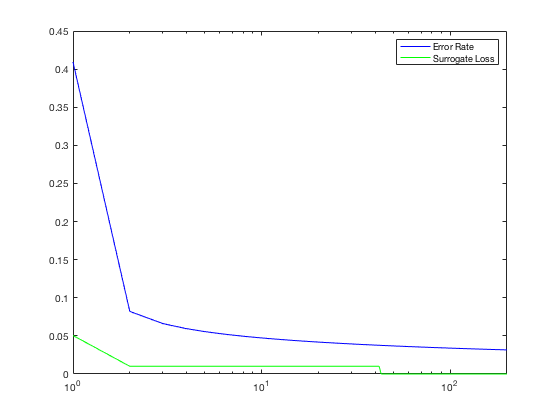
\includegraphics[width=30em,keepaspectratio]{p5figure7.png}\\
	{Figure 2.5.7: Surrogate loss and error rate for data set A}
	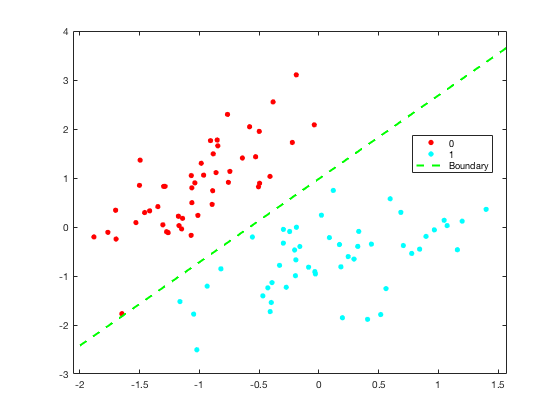
\includegraphics[width=30em,keepaspectratio]{p5figure8.png}\\
	{Figure 2.5.8: Final converged classifier for data set A}
		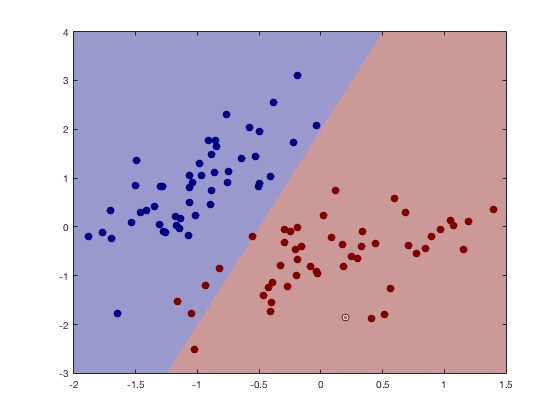
\includegraphics[width=30em,keepaspectratio]{p5figure9.png}\\
	{Figure 2.5.9: Classes and decision boundary plotted using plotClassify2D for data set A}
	
		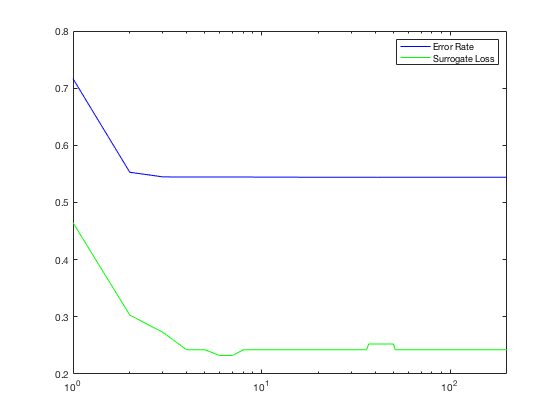
\includegraphics[width=30em,keepaspectratio]{p5figure10.png}\\
	{Figure 2.5.10: Surrogate loss and error rate for data set B}
	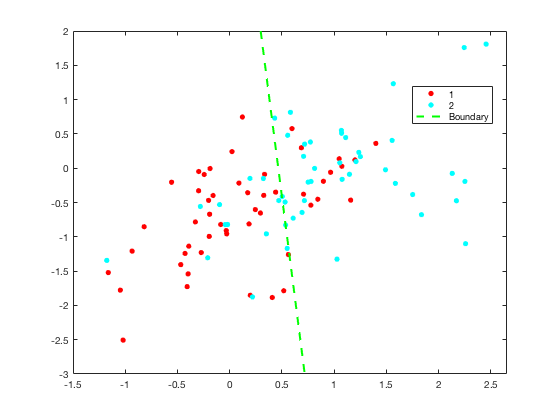
\includegraphics[width=30em,keepaspectratio]{p5figure11.png}\\
	{Figure 2.5.11: Final converged classifier for data set B}
	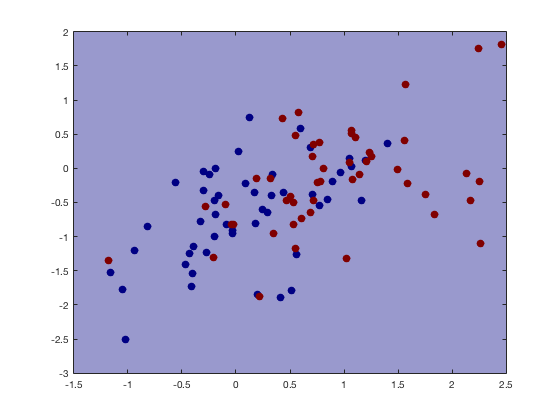
\includegraphics[width=30em,keepaspectratio]{p5figure12.png}\\
	{Figure 2.5.12: Classes and decision boundary plotted using plotClassify2D for data set B}
\end{center} 

\lstinputlisting[language=Matlab]{MATLABfiles/@logisticClassify2/train.m}

\bigbreak
\textbf{(g) To implement the mini batch gradient descent on the logistic function complete your train$\_$in$\_$batches.m function. This will require that you :}
\smallbreak
\textbf{(1) fill in create$\_$mini$\_$batches.m function, which generates the mini batches of data. shuffle your data inside this function and set the batch size to 11;}

\lstinputlisting[language=Matlab]{MATLABfiles/@logisticClassify2/create_mini_batches.m}
\bigbreak
\textbf{(2) update the training iterations in train$\_$in$\_$batches.m, in contrast to the training in section (e), in this function training will be performed on each of these data batches;}
\lstinputlisting[language=Matlab]{MATLABfiles/@logisticClassify2/train_in_batches.m}
\bigbreak
\textbf{(3) change the training method in logisticClassify2 (set it into "train$\_$in$\_$batches") and run your mini batch logistic regression classifier. In your report please include the functions that you wrote create$\_$mini$\_$batches.m and train$\_$in$\_$batches.m)}
\begin{lstlisting}[language=Matlab]
% Train Set A
train_in_batches(learner, XA, YA,11, 'stopIter', 100, 'stepsize', 0.1);
legend('Error Rate', 'Surrogate Loss');
% Plot final converged classifier decision boundaries.
figure();
plotClassify2D(learner, XA, YA);

%% Train Set B
figure
train_in_batches(learner, XB, YB,11, 'stopIter', 100, 'stepsize', 0.1);
legend('Error Rate', 'Surrogate Loss');
% Plot final converged classifier decision boundaries.
figure();
plotClassify2D(learner, XB, YB);
\end{lstlisting}
\begin{center}
	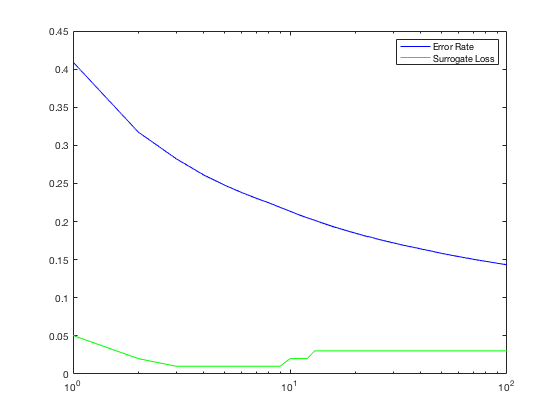
\includegraphics[width=30em,keepaspectratio]{p5figure13.png}\\
	{Figure 2.5.13: Surrogate loss and error rate for data set A trained in minibatches}
	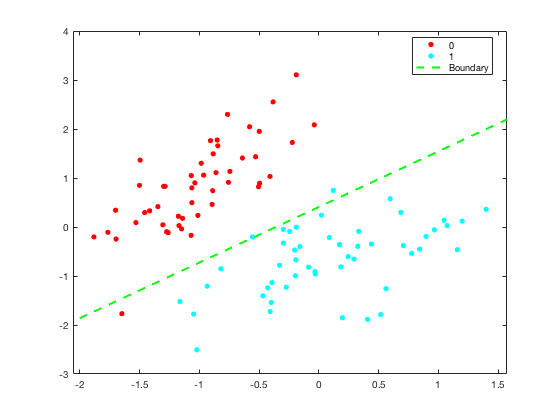
\includegraphics[width=30em,keepaspectratio]{p5figure14.png}\\
	{Figure 2.5.14: Final converged classifier for data set A trained in minibatches}
	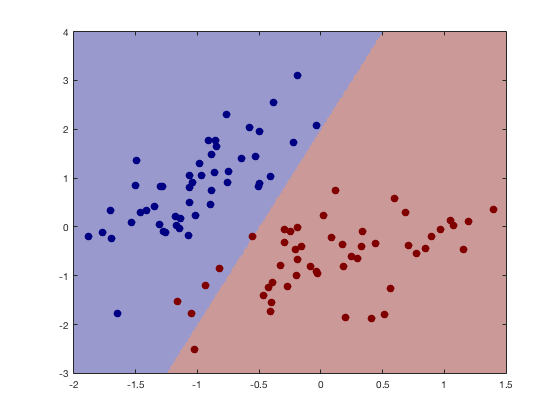
\includegraphics[width=30em,keepaspectratio]{p5figure15.png}\\
	{Figure 2.5.15: Classes and decision boundary plotted using plotClassify2D for data set A trained in minibatches}
	
	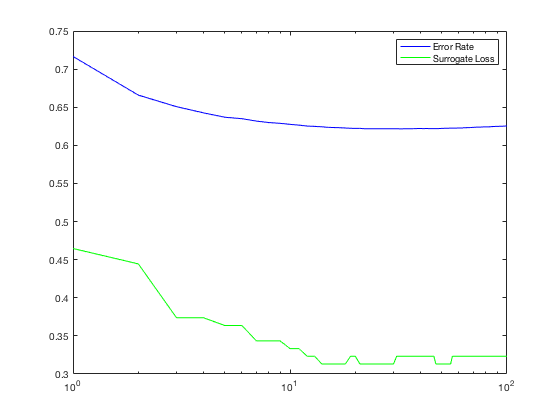
\includegraphics[width=30em,keepaspectratio]{p5figure16.png}\\
	{Figure 2.5.16: Surrogate loss and error rate for data set B trained in minibatches}
	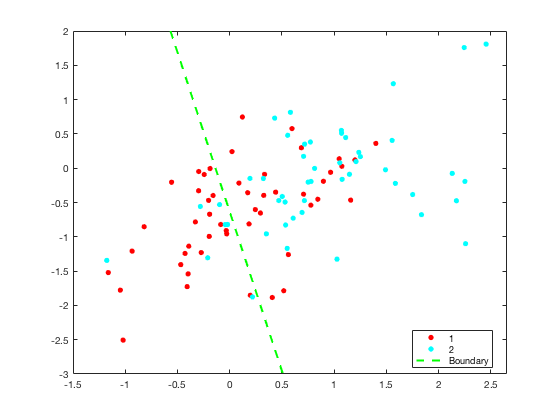
\includegraphics[width=30em,keepaspectratio]{p5figure17.png}\\
	{Figure 2.5.17: Final converged classifier for data set B trained in minibatches}
	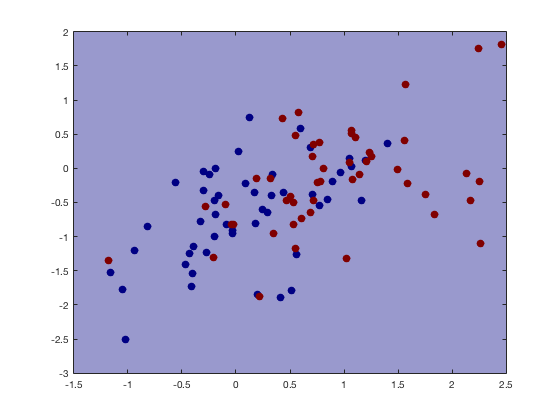
\includegraphics[width=30em,keepaspectratio]{p5figure18.png}\\
	{Figure 2.5.18: Classes and decision boundary plotted using plotClassify2D for data set B trained in minibatches}
\end{center} 

\end{document}
